La desintegración en cadena  del $^{235} U$ se conoce como la serie del actínido \cite{Podgorsak.2016}. Como parte del proceso de desintegración radiactiva, los productos de fisión del uranio emiten neutrones y rayos gamma al atravesar una serie de decaimientos beta \cite{Guo.2016}. La causa de esta serie de desintegraciones nucleares se debe a la razón de neutrones sobre protones, es mediante el canal beta que estos núcleos logran la estabilidad \cite{Guo.2016}. 

De acuerdo con \textit{Guo et al, 2016}, al momento de analizar una cadena de desintegración compleja se simplifica el problema al resolver la reacción a través de reacciones lineales en las que cada núcleo está relacionado solo a un núcleo madre; el núcleo madre puede estar en su estado base o en un estado excitado, partiendo de esto llamamos a cada cadena lineal \textit{la del estado base} y \textit{la del estado excitado}, respectivamente.

El proceso de desintegración del uranio-235 contempla bifurcaciones en varios puntos, esto es: hay productos de desintegración que pueden a su vez producir uno de dos posibles núcleos más estables \cite{HUBENER2003211, International_Atomic_Energy_Agency2013-bq}. La literatura observa más o menos bifurcaciones para el proceso, como podemos apreciar en \cite{HUBENER2003211,International_Atomic_Energy_Agency2013-bq,Pratiwi.2021,Loch.2013}, por mencionar tres ejemplos. Para mantener la simulación lo más fiel posible al proceso real, tomamos como referencia la cadena presentada por \textit{Hübener} en \cite{HUBENER2003211}, la cual está ilustrada en la imagen \ref{cadenadelu235}.

\begin{figure}[H]
    \centering
    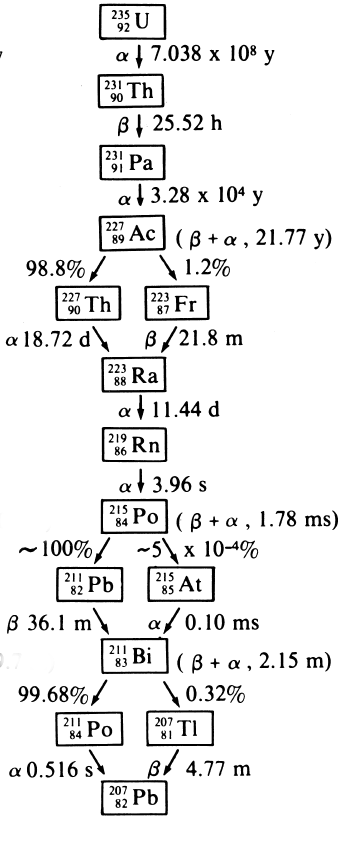
\includegraphics[scale=0.425]{imagenes/cadenaluz.png}
    \caption{Cadena de desintegración del U235 hasta Pb207. Tomada de \cite{HUBENER2003211}}.
    \label{cadenadelu235}
\end{figure}

Contemplar el proceso de enriquecimiento del material fisionable complica en gran manera la resolución del problema, es por esto que ignoraremos esta etapa del proceso.  

\subsection{Ecuaciones de Bateman para la serie del actínido}

Es posible modelar las ecuaciones de Bateman en una notación matricial contemplando un sistema de ecuaciones para cada posible bifurcación \cite{Pratiwi.2021}. Nuestra intención en este estudio es más bien contemplar las bifurcaciones mediante un modelo diferencial estocástico.

Tomando en cuenta las condiciones iniciales \ref{condicioninicialpadre} y \ref{condicioninicialproductos} y la forma de $N_i(t)$ en \ref{iesimonucleo}, podemos plantear las ecuaciones de Bateman de la siguiente forma:
\begin{align}
    N_1'(t)&=-\lambda_1 N_1(t)\\ \label{ecubateman1} %Uranio
    N_2'(t)&=\lambda_1 N_1(t) -\lambda_2 N_2(t)\\ %Torio
    N_3'(t)&=\lambda_2 N_2(t) -\lambda_3 N_3(t)\\ %Paladio
    N_4'(t)&=\lambda_3 N_3(t) -\lambda_4 N_4(t)\\ %Actinio
    N_5'(t)&=(1-f_4)\lambda_4 N_4(t) -\lambda_5 N_5(t)\\ %Torio
    N_6'(t)&=f_4 \lambda_4 N_4(t) -\lambda_6 N_6(t)\\ %Francio
    N_7'(t)&=\lambda_5 N_5(t) + \lambda_6 N_6(t) -\lambda_7 N_7(t)\\ %Radio
    N_8'(t)&=\lambda_7 N_7(t) -\lambda_8 N_8(t)\\ %Radón
    N_9'(t)&=\lambda_8 N_8(t) -\lambda_9 N_9(t)\\ %Polonio
    N_{10}'(t)&=f_9\lambda_9 N_9(t) -\lambda_{10} N_{10}(t)\\ %Plomo
    N_{11}'(t)&=(1-f_9)\lambda_9 N_9(t) -\lambda_{10} N_{11}(t)\\ %Astato
%\end{align}
%
%\begin{align}
   \nonumber N_{12}'(t)&=\lambda_{10} N_{10}(t) +\lambda_{11} N_{11}(t)\\
   &-\lambda_{12} N_{12}(t)\\ %Bismuto
    N_{13}'(t)&=(1-f_{12})\lambda_{12} N_{12}(t) -\lambda_{13} N_{13}(t)\\ %Polonio
    N_{14}'(t)&=f_{12}\lambda_{12}N_{11}(t) -\lambda_{14} N_{14}(t)\\ %Talio
    N_{15}'(t)&=\lambda_{13} N_{13}(t) + \lambda_{14} N_{14}(t) %Plomo
    \label{ecubateman15}
\end{align}

\noindent donde $f_k$ son tasas de ramificación. Las $N_i(t)$ se definen de la siguiente manera:
\begin{itemize}
    \item $N_1(t)\equiv$ \textit{Núcleos de} $^{235}U$.
    \item $N_2(t)\equiv$ \textit{Núcleos de} $^{231}Th$.
    \item $N_3(t)\equiv$ \textit{Núcleos de} $^{231}Pa$.
    \item $N_4(t)\equiv$ \textit{Núcleos de} $^{227}Ac$.
    \item $N_5(t)\equiv$ \textit{Núcleos de} $^{227}Th$.
    \item $N_6(t)\equiv$ \textit{Núcleos de} $^{223}Fr$.
    \item $N_7(t)\equiv$ \textit{Núcleos de} $^{223}Ra$.
    \item $N_8(t)\equiv$ \textit{Núcleos de} $^{219}Rn$.
    \item $N_9(t)\equiv$ \textit{Núcleos de} $^{215}Po$.
    \item $N_{10}(t)\equiv$ \textit{Núcleos de} $^{211}Pb$
    \item $N_{11}(t)\equiv$ \textit{Núcleos de} $^{215}At$.
    \item $N_{12}(t)\equiv$ \textit{Núcleos de} $^{211}Bi$.
    \item $N_{13}(t)\equiv$ \textit{Núcleos de} $^{211}Po$.
    \item $N_{14}(t)\equiv$ \textit{Núcleos de} $^{207}Tl$.
    \item $N_{15}(t)\equiv$ \textit{Núcleos de} $^{207}Pb$.
\end{itemize}

\noindent para los factores de ramificación tenemos:
\begin{itemize}
    \item $f_4=\frac{\lambda_{4,\alpha}}{\lambda_{4,\alpha}+\lambda_{4,\beta}}$, donde $\lambda_{4,\alpha}$ es la tasa de desintegración del $^{227}Ac$ hacia $^{223}Fr$, mientras que $\lambda_{4,\beta}$ representa la tasa de desintegración de $^{227}Ac$ hacia $^{227}Th$. 
    \item $f_9=\frac{\lambda_{9,\alpha}}{\lambda_{9,\alpha}+\lambda_{9,\beta}}$, donde $\lambda_{9,\alpha}$ es la tasa de desintegración del $^{215}Po$ hacia $^{211}Pb$, mientras que $\lambda_{9,\beta}$ representa la tasa de desintegración de $^{215}Po$ hacia $^{215}At$.
    \item $f_{12}=\frac{\lambda_{12,\alpha}}{\lambda_{12,\alpha}+\lambda_{12,\beta}}$, donde $\lambda_{12,\alpha}$ es la tasa de desintegración del $^{211} Bi$ hacia $^{207} Tl$, mientras que $\lambda_{12,\beta}$ representa la tasa de desintegración de $^{211} Bi$ hacia $^{211} Po$.
\end{itemize}

Las tasas de ramificación pueden verse como una medida de probabilidad para la ocurrencia de un canal de desintegración. 

De acuerdo con los archivos de \textit{National Nuclear Data Center} en la base de datos \textit{NuDat}, las probabilidades para el canal alfa y el beta en el Ac-227 son, respectivamente, 0.013800 y 0.98620; para el canal alfa y beta en el Po-215 son, respectivamente, 0.9999977 y 0.0000023; para el canal alfa y el beta en el Bi-211 son, respectivamente, 0.99724 y 0.00276. De manera que $f_4=0.01380$, $f_9=0.9999977$ y $f_{11}=0.99724$.

La constante de decaimiento $\lambda_i$ para el i-ésimo núcleo depende del período de semi-desintegración $T_{1/2}^{(i)}$, estos valores son conocidos y están documentados en la literatura, tal es el caso de \cite{Flanagan1954} y la base datos \textit{NuDat}. La tabla \ref{tabladeconstantesdedesintegracion} muestra las constantes de decaimiento de cada núcleo en las ecuaciones \ref{ecubateman1} hasta \ref{ecubateman15} junto con el período de semi-desintegración que le concierne según \textit{NuDat} por estar más actualizado. 

Lo que no se muestra en la tabla \ref{tabladeconstantesdedesintegracion} es las constantes de decaimiento correspondientes a los canales específicos $\alpha$ y $\beta$ en la desintegración del $^227 Ac$, $^215 Po$, y $^211 Bi$. De la definición de razón de fraccionamiento, se puede deducir que

$$\lambda_{4,\alpha}=0.4394\times 10^{-3}\unit{a^{-1}}$$
$$\lambda_{4,\beta}=3.140\times 10^{-3}\unit{a^{-1}}$$
$$\lambda_{9,\alpha}=1.227\times 10^{10}\unit{a^{-1}}$$
$$\lambda_{9,\beta}=2.822\times 10^{4}\unit{a^{-1}}$$
$$\lambda_{11,\alpha}=2.180\times 10^{11}\unit{a^{-1}}$$
$$\lambda_{11,\beta}=6.033\times 10^{8}\unit{a^{-1}}$$

%\begin{minipage}{\textwidth}
%\begin{table}[h]
%    \centering
\begin{center}
\noindent\begin{tabular}{|c|l|l|}
\hline
Radionúclido & \multicolumn{1}{c|}{$T_{1/2}$} & \multicolumn{1}{c|}{$\lambda\ (a^{-1})$} \\\hline\hline 
$^{235}U$  & $\unit[7.04\times 10^8]{a}$ & $9.846\times 10^{-10}$ \\
$^{231}Th$ & $\unit[25.52]{h}$ & $1.786\times 10^{-3}$ \\
$^{231}Pa$ & $\unit[3.276\times 10^4]{a}$ & $2.116\times 10^{-5}$ \\
$^{227}Ac$ & $\unit[21.772]{a}$ & $3.184\times 10^{-2}$ \\
$^{227}Th$ & $\unit[18.697]{d}$ & $1.353\times 10^{1}$ \\
$^{223}Fr$ & $\unit[22.00]{min}$ & $1.656\times 10^{4}$ \\
$^{223}Ra$ & $\unit[11.43]{d}$ & $2.213\times 10^{1}$ \\
$^{219}Rn$ & $\unit[3.96]{s}$ & $5.520\times 10^{6}$ \\
$^{215}Po$ & $\unit[1.781\times 10^{-3}]{s}$ & $1.227\times 10^{10}$ \\
$^{211}Pb$ & $\unit[36.1]{min}$ & $1.009\times 10^{4}$ \\
$^{215}At$ & $\unit[0.10\times 10^{-3}]{s}$ & $2.186\times 10^{11}$ \\
$^{211}Bi$ & $\unit[2.14]{min}$ & $1.702\times 10^{5}$ \\
$^{211}Po$ & $\unit[0.516]{s}$ & $4.236\times 10^{7}$ \\
$^{207}Tl$ & $\unit[4.77]{min}$ & $7.638\times 10^{4}$ \\
$^{207}Pb$ & Estable & \\\hline
\end{tabular}
\captionof{table}{Períodos de semidesintegración y constantes de decaimiento para cada radionúclido en la cadena del uranio-235. Datos según \textit{NuDat}.}
\label{tabladeconstantesdedesintegracion}
%\end{table}
%\end{minipage}
\end{center}

Hay que señalar que en este modelo, las ecuaciones de Bateman tienen una forma determinista. Bajo la perspectiva de un modelo estocástico diferencial, vemos que la solución del sistema sería la solución esperada para el caso determinista más un término perturbativo que es en sí una variable aleatoria dependiente del tiempo. 

En la literatura se reportan métodos analíticos para resolver sistemas de ecuaciones como el planteado aquí empleando transformadas de Laplace o exponenciales de matrices. En el presente, utilizamos el método de eigenvectores para establecer la solución general del sistema. Al notar que el sistema de ecuaciones puede representarse con una ecuación matricial de la forma

$$\mathbf{N'}(t)=\Lambda \mathbf{N}(t)$$

Donde $\mathbf{N}(t)$ es un vector cuyas componentes son las funciones $N_i(t)$ y $\mathbf{N'}(t)$ es el vector que contiene sus derivadas. La matriz $\Lambda$ es triangular inferior de dimensión $14\times14$, dada como \ref{matriz_determinista} en los anexos.

De tal forma que las soluciones del sistema vienen dados como combinación lineal de los eigenvectores de $\Lambda$:

$$\mathbf{N}(t)=\kappa_1 e^{-\lambda_1 t} \mathbf{V}_{\lambda_1}+\kappa_2 e^{-\lambda_2 t} \mathbf{V}_{\lambda_2}+...+\kappa_{14} e^{-\lambda_{14} t} \mathbf{V}_{\lambda_{14}}$$

\noindent Las constantes de integración $K_i$ son determinadas por las condiciones iniciales $\mathbf{N}(0)=\left[N_1^{(0)}\ 0\ 0\ ...\ 0\right]^T$.

\subsubsection{Cálculo de los coeficientes de Bateman}

De acuerdo con la ecuación \ref{batemangeneral}, podemos emplear las constantes de decaimiento en el cuadro \ref{tabladeconstantesdedesintegracion} para determinar los coeficientes de Bateman de la serie del actínido. Resumimos los resultados en el cuadro \ref{tabla_coeficientes_bateman1} y \ref{tabla_coeficientes_bateman2}. Donde $C_k^*=C_k/N_1^{(0)}$. Estos resultados han de reemplazarse en las soluciones deterministas para trazar las gráficas del decaimiento de cada una de las muestras resultantes en la cadena, así como del núcleo padre. Al encontrar las soluciones deterministas tenemos un acercamiento al perfil que tendrán las soluciones estocásticas. 

Por otro lado, los coeficientes obtenidos en el método de eigenvectores están resumidos en el cuadro \ref{tabladecoeficientes2}. 

\begin{center}
\begin{tabular}{|c|r|}
    \hline
    k-ésimo coeficiente & \multicolumn{1}{c|}{valor aproximado}\\\hline\hline
    $\kappa_1^*$ & 1.000 \\
    $\kappa_2^*$ & $-1.7112\times 10^{-32}$ \\
    $\kappa_3^*$ & $6.7401\times 10^{-34}$ \\
    $\kappa_4^*$ & $-1.5322\times 10^{-30}$ \\
    $\kappa_5^*$ & $-3.1814\times 10^{-29}$ \\
    $\kappa_6^*$ & $4.3028\times 10^{-42}$ \\
    $\kappa_7^*$ & $-4.0795\times 10^{-35}$ \\
    $\kappa_8^*$ & $2.6946\times 10^{-32}$ \\
    $\kappa_9^*$ &  $6.7765\times 10^{-24}$ \\
    $\kappa_{10}^*$ & $1.5548\times 10^{-24}$ \\
    $\kappa_{11}^*$ & $1.3446\times 10^{-29}$ \\
    $\kappa_{12}^*$ & $-1.7296\times 10^{-12}$ \\
    $\kappa_{13}^*$ & $-6.6619\times 10^{-5}$\\
    $\kappa_{14}^*$ & $-7.8436\times 10^{-7}$ \\
    $\kappa_{15}^*$ & $1.4142$\\
    \hline
\end{tabular}
\captionof{table}{Coeficientes de Bateman mediante método de eigenvectores.}\label{tabladecoeficientes2}
\end{center}

\subsection{Modelo estocástico matricial}
Un modelo estocástico matricial del sistema se puede construir usando una matriz determinista alternativa $\mathcal{L}$ más tres matrices $\mathcal{X}$, $\mathcal{Y}$ y $\mathcal{Z}$ que conjuntamente representan un ruido estocástico sobre $\mathcal{L}$. El sistema matricial es

\begin{equation}
	\mathcal{N}'(t)=(\mathcal{L}+x\mathcal{X}+y\mathcal{Y}+z\mathcal{Z})\mathcal{N}(t)
\end{equation}

\noindent donde los parámetros $x, y,\textrm{ y }z$ son variables aleatorias discretas que pueden ser 0 o 1, no necesariamente todas a las vez, y dictan la ocurrencia de una bifurcación en la cadena. La forma explícita de estos cuatro arreglos puede verse en los anexos en las ecuaciones \ref{matriz_determinista_alternativa}, \ref{matriz_estocastica_x}, \ref{matriz_estocastica_y} y \ref{matriz_estocastica_z}. El vector $\mathcal{N}$ corresponde al vector de funciones del número de núcleos por unidad de tiempo para cada especie química en la cadena bajo el esquema estocástico. 